\section{Introduction}

\lettrine{T}he comparison of the aerodynamic efficiency of gliding birds against the UAVs is insightful for a better understanding of natural flight. There has been an increased recognition that more attention needs to be paid to morphing wings. Wing morphing allows gulls to modulate static pitch stability during gliding \cite{Harvey2022BirdsMorphing}. 
The morphing ability of the flexible membrane wing is provided by its flexibility, which allows it to alter shape adaptively under aerodynamic loading. The aerodynamic performance modeling and flow control are drawing the interest of zoologists, biologists, and the concerned aerodynamics community. As a result, these researches combine the biological theory of natural flying with aerodynamic methodologies to address MAVs based on bird endurance. Flexible wing is a successful way for improving the aerodynamic robustness of tiny fixed wing drones operating in uncertain air situations by using a revolutionary biomimetic design.
The aim is to introduce a multidisciplinary approach to the study of biologically influenced flights by coupling aerodynamics, structure, and flight mechanics.

The birds wing aerodynamic is different in behavior compared to the conventional man-made wings as \citet{Withers1981} found that the bird wings perform with low drag generally had low maximum lift coefficients whereas wings with high maximum lift coefficients had high drag coefficients. 
Their wings are models for the construction as noise reducing application \cite{Bachmann2010}.
Early studies on experimental biology focused on the material properties testing of the biological flights such as the wings and feathers structures \cite{Bachmann2012}.
Among the studied species is the owl. They are known for their silent flight because of the features in its wings that promote smooth flow \cite{Jaworski2020,Wagner2017,Geyer2016}. 
Implementation of biomimetic approach is meant to replicate the feather effects on aerodynamic performance \cite{Hedenstrom2017}. 
%
A thin and feather-like shapes that have a finite trailing edge thickness were designed by \citet{Ananda2018} by using a multipoint inverse airfoil design technique in PROFOIL \cite{AirfoilDesignSoftwarefortheWeb} to design airfoil families (AS6091 to AS6099).
%
It consists of modifications in the finite trailing thickness between 4\%–6\% and can perform efficiently at the same bird Reynolds number scales ($10^4$–$10^5$).
%

\\
\subsection{Previous work}

\citet{Harvey2022AControl} focused their survey on various possible control provided by bio-inspired morphing that engineering studies could validate and incorporate to enhance flight maneuverability. Using morphing mechanisms including camber morphing techniques, wing morphing can be utilized to alter lift distributions and generate longitudinal control (Fig.\ref{fig:camberMorphing} . A deeper understanding of their control response in dynamic and turbulent environments is required concluded the review.
This camber-morphing airfoil method extends prior work by its unique consideration of the instantaneous flow control \citet{Gamble2020a,Gamble2020b}.

\\

\begin{figure}[hbt!]
  \centering
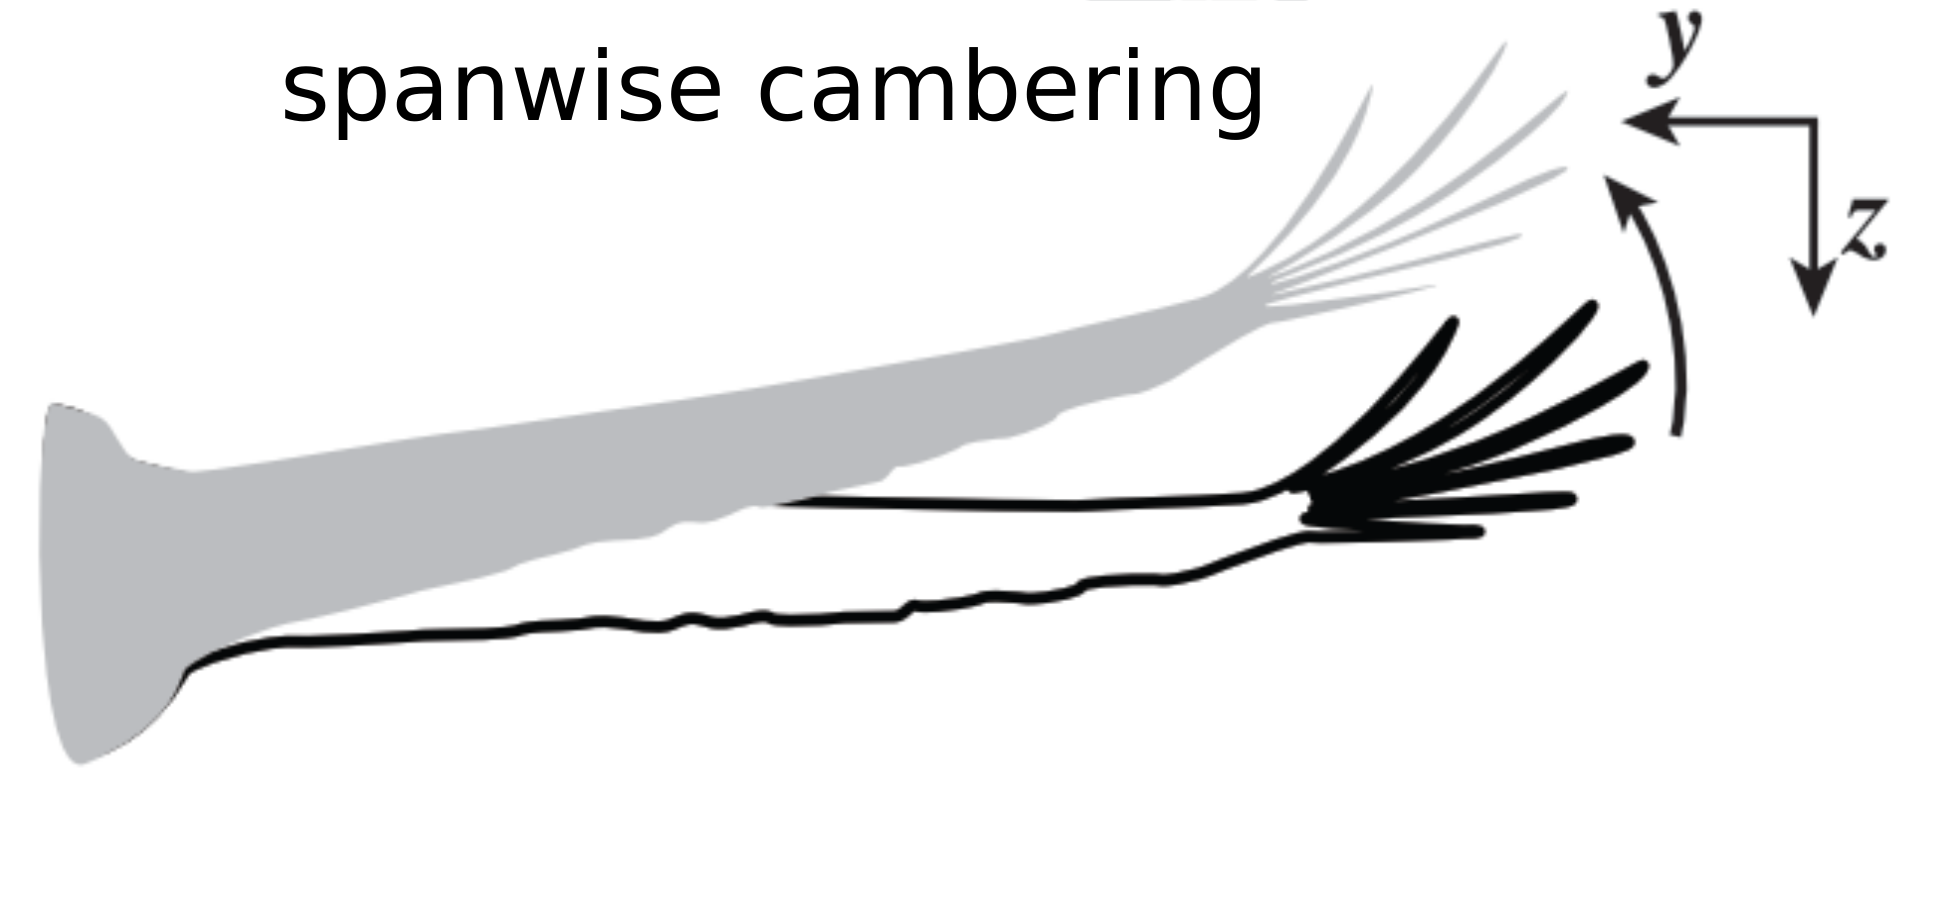
\includegraphics[width=2.5in]{Figures/span morphing.png}
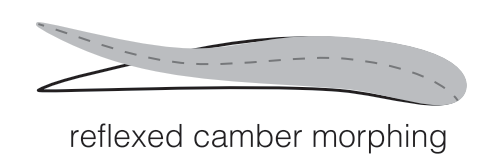
\includegraphics[width=2.5in]{Figures/camber morphing.png}
  
  \caption{\label{fig:camberMorphing} Different UAV implementations of avian-inspired wing camber morphing spanwise cambering and chordwise morphing \cite{Harvey2022AControl} }
\end{figure}



Although some attempts have been made to address morphing wings, much of the work in this area is limited to steady CFD predictions of the original and morphing airfoils.

As a first step to understanding how the flow responds to dynamic morphing flap deflection,  insightful work is presented by \cite{Abdessemed2018MorphingMeshing} using dynamic meshing to perform CFD analyses. The NACA 0012 airfoil fitted with a morphing trailing edge (TE) flap showed to have potential for future applications. 

Here it is reported that those studies neglected dynamic aspect of the interaction between fluid and wings.

In these directions, a growing field of researchers studying and developing avian-inspired morphing aircraft focused on the study of the morphing wings. \citet{Gamble2020a} found that the bio inspired flexible airfoil maintained lift at Reynolds numbers below 1.5x$10^5$, but at greater Reynolds numbers, the flexible airfoil alleviated the lift force and experienced trailing edge displacement.

\citet{Murayama2021} in their study showed the effectiveness of flexible flaps inspired by bird feathers can improve aerodynamic robustness in low Reynolds number wings. It reduces the fluctuations of aerodynamic forces in a perturbed flow behind an oscillating plate by suppressing large-scale vortex shedding. 
In previous work on understanding the low Re aerodynamic phenomena encountered while studying the owl-like airfoil \cite{Boughou2022} showed the unsteadiness of the aerodynamic coefficients. The aero-structural response to the aerodynamic load is the motive behind the work presented in this paper.

\subsection{Objectives}
The role of feather morphing hasn't been thoroughly investigated, and its impact on aerodynamics is unknown. 
The aero-structural response of a flexible airfoil designed using biologically inspired structural and material data from feathers requires studies that to concentrate on evaluating aerodynamic load the aero-structural features in turbulent situations. In the current study on bio-inspired flexible wings, we aim to make use of existing research in the field and complete several objectives. 

First, we examine bio-inspired structure requirements  necessary to capture both flow field and structural analysis. 
Computational modeling can provide a way to develop predictive relationships between morphological traits and their impact on aerodynamic performance through a series of flexibility conditions will be computed using Fluid-Structure interaction (FSI).
One of the primary objectives of evaluations is to investigate the dynamic interaction between Low Re aerodynamic flow and Flexible-Biomimetic NACA6409 as earlier recommended in Ref \cite{Gamble2020b} at an angle of attack 15$^{\circ}$. 
Furthermore, the secondary goal of the study is to investigate  and assess  feather-like airfoils that resemble a cross-section of a bird wing \cite{Murayama2021}, which are narrow plate-like feather that expand toward the trailing edge will be performed. 